\documentclass[11pt]{article}
\usepackage[letterpaper, margin=1in]{geometry}
\usepackage{amsmath, amssymb, amsthm, mathtools, bm}
\usepackage{graphicx}
\graphicspath{{../figures/}}
\usepackage{booktabs, multirow}
\usepackage[round, authoryear]{natbib}
\usepackage[dvipsnames]{xcolor}
\usepackage{microtype}
\usepackage{algorithm}
\usepackage[noend]{algorithmic}
\usepackage[font=small, labelfont=bf, skip=4pt]{caption}
\usepackage{enumitem}
\usepackage[colorlinks=true, linkcolor=MidnightBlue, citecolor=MidnightBlue, urlcolor=MidnightBlue]{hyperref}
\usepackage[capitalise, noabbrev]{cleveref}

\setlist{itemsep=1pt, topsep=3pt}
\renewcommand{\algorithmicrequire}{\textbf{Input:}}
\renewcommand{\algorithmicensure}{\textbf{Output:}}
\newtheorem{proposition}{Proposition}

\newcommand{\R}{\mathbb{R}}
\newcommand{\tr}{\operatorname{tr}}
\newcommand{\prox}{\operatorname{prox}}
\newcommand{\nmse}{\mathrm{nMSE}}
\newcommand{\one}{\mathbf{1}}
\DeclareMathOperator*{\argmin}{arg\,min}


\title{\textbf{Shrink Towards the Mean, Not Towards Zero:\\ Revisiting Pooling Baselines for Regularized\\ Multi-Task Learning on the School Benchmark}}
\author{
  Devangan Mukherjee\\[2pt]
  Department of Metallurgical and Materials Engineering\\
  Indian Institute of Technology Kharagpur, India\\
  \texttt{devanganrox007@gmail.com}
}
\date{October 2026}

\begin{document}
\maketitle

\begin{abstract}
Regularized multi-task learning (MTL) is usually judged against independent per-task models. On the School benchmark (139 schools, 15,362 students), the opposite extreme, a single model pooled across all schools, has mostly been reported under a 75\% training protocol, with conflicting conclusions: it was the best method of \citet{evgeniou2005kernel} and clearly behind multi-task feature learning in \citet{argyriou2008convex}. We revisit this comparison across training fractions, with a focus on the low-data regime. A short NumPy implementation first reproduces published results, matching the trace-norm explained variance of \citet{argyriou2008convex} (26.5\% against 26.7\%). Across training fractions from 5\% to 75\% of each school, trace-norm MTL beats independent ridge on every split, by 19.2\% in normalized mean squared error at 5\% and 4.4\% at 75\%, yet the pooled model beats it on every split up to 20\%. Two facts explain the reversal. School-level covariates are constant within each school, so their effects are identifiable only across schools, and the trace-norm and $\ell_{2,1}$ penalties shrink every school towards zero: at 5\% the average trace-norm school model has 57\% of the norm of the pooled model. Mean-regularized MTL, which learns a shared mean and penalizes only deviations from it, stays within 0.4\% of pooled ridge at 5\%, beats it on every split from 10\% onwards by up to 6.3\%, and has lower error than trace-norm MTL at every training fraction; constraining the deviations to be low rank adds nothing on this benchmark. We also show that a fixed iteration budget fails silently on unscaled features, and that two common definitions of explained variance differ by 11 to 13 points for identical predictions.

\end{abstract}

\section{Introduction}
\label{sec:intro}

Multi-task learning (MTL) fits several related prediction problems together so that problems with few examples can borrow statistical strength from the others \citep{caruana1997multitask, zhang2022survey}. In its linear form, the relationship between tasks is encoded as a regularizer on the matrix of task weights: a trace norm when tasks are believed to share a low-dimensional subspace, an $\ell_{2,1}$ norm when they share a subset of features, or a learned task covariance \citep{argyriou2008convex, obozinski2010joint, zhang2010convex}. These methods are usually evaluated against the opposite extreme, one independent model per task, and the size of the improvement over that baseline is taken as the value of sharing.

There is a second extreme that receives much less attention: a single model fitted to all tasks at once. Multilevel statistics calls the two extremes \emph{no pooling} and \emph{complete pooling}, and the standard recommendation is \emph{partial pooling}, which shrinks each group's estimate towards a common one by an amount learned from the data \citep{gelman2007data}. If tasks share most of their structure, complete pooling can be a strong competitor, and it is strongest precisely where MTL is advertised to help most: when each task has little data.

We study this question on the School benchmark, a set of 139 regression tasks (one per London secondary school) that has served as a standard test of multi-task methods for two decades \citep{bakker2003task, evgeniou2005kernel, argyriou2008convex}. Our study is deliberately small and fully reproducible. It uses one dataset, linear models and squared loss, so that every effect can be traced to a cause. \Cref{fig:overview} previews the central contrast.

On School, the pooled baseline has a mixed record. \citet{evgeniou2005kernel} found that one support vector machine fitted to all schools performed best, ahead of both independent and multi-task kernels, whereas \citet{argyriou2008convex} reported the aggregate model well below multi-task feature learning. Both comparisons use the same, largest training fraction (75\% of each school), where school-specific models are at their strongest. Partial pooling is equally classical: mean-regularized MTL shrinks every task towards a learned common model \citep{evgeniou2004regularized}, and recent theory shows that estimators of this kind adapt to the unknown similarity between tasks, behaving like pooling when tasks are alike and like independent fitting when they are not \citep{duan2023adaptive}. None of these estimators is new. Our contribution is empirical: we measure where on the data-size axis each regime holds on School, and explain why.

\begin{figure}[t]
\centering
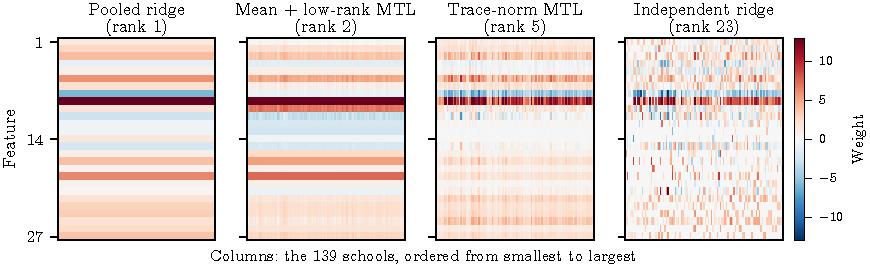
\includegraphics[width=\textwidth]{fig1_model_matrices.pdf}
\caption{Learned model matrices $W$ on School at $\rho = 20\%$ (first split), intercept row omitted; each column is one school's model, schools ordered by size. Pooled ridge uses one model for every school (rank 1), and independent ridge fits each school alone (rank 23). Trace-norm MTL shares a subspace but pales the shared weights, shrinking them towards zero. Mean + low-rank MTL, one of the two partial-pooling estimators we study, keeps the pooled weights and adds small structured deviations.}
\label{fig:overview}
\end{figure}

\paragraph{Contributions.}
\begin{itemize}[leftmargin=*]
\item \textbf{Reproduction.} With a short NumPy implementation of proximal-gradient MTL, we reproduce published School results under two protocols, matching the trace-norm result of \citet{argyriou2008convex} to within 0.2 points of explained variance (\cref{sec:res-repro}).
\item \textbf{Pooling across data sizes.} Over training fractions from 5\% to 75\% of each school, trace-norm MTL beats independent ridge on every split, yet a single pooled ridge model beats it on every split up to 20\% (\cref{sec:res-curves}). We trace this to the data, in which school-level covariates are constant within each school, and to the regularizers, which shrink towards zero rather than towards a common model (\cref{sec:res-why}, \cref{prop:limits}).
\item \textbf{Partial pooling.} Mean-regularized MTL, which learns a shared mean and penalizes only deviations from it, stays within 0.4\% of pooled ridge at 5\% training and is the best or tied-best method from 10\% onwards; constraining the deviations to be low rank does not help (\cref{sec:res-partial}). Its advantage over trace-norm MTL is largest for small schools (\cref{sec:res-who}).
\item \textbf{Evaluation pitfalls.} A fixed iteration budget fails silently on unscaled features, and two common definitions of explained variance differ by 11 to 13 points for identical predictions (\cref{sec:res-optim,sec:res-metrics}).
\end{itemize}

\section{Related Work}
\label{sec:related}

\paragraph{Regularized multi-task learning.}
Multi-task learning trains related predictors jointly so that tasks with little data borrow strength from the rest \citep{caruana1997multitask}; see \citet{zhang2022survey} and \citet{yu2024unleashing} for surveys. In the linear setting the coupling is usually a regularizer on the matrix of task weights. \citet{evgeniou2004regularized} penalize the distance of each task to a shared mean. \citet{argyriou2008convex} learn a shared low-dimensional representation and show that their convex formulation is equivalent to trace-norm regularization; the $\ell_{2,1}$ norm instead selects a common subset of features \citep{obozinski2010joint, liu2009multitask}. Decomposition models add a task-specific component to a shared one, giving ``dirty'' models with sparse deviations \citep{jalali2010dirty, chen2012incoherent} and robust models that isolate outlier tasks \citep{chen2011integrating}. Other work learns the task relationships themselves, as a task covariance \citep{zhang2010convex} or as overlapping groups through a shared basis \citep{kumar2012learning}. Proximal gradient methods with Nesterov acceleration \citep{beck2009fista, ji2009accelerated} are the standard solvers, and the MALSAR toolbox \citep{zhou2011malsar} packages many of these formulations together with the School data used here.

\paragraph{The School benchmark.}
The Inner London Education Authority examination data, with one regression task per secondary school, became a standard multi-task benchmark through \citet{bakker2003task} and \citet{evgeniou2005kernel}, and has been reported under several protocols since \citep{argyriou2008convex, zhang2010convex, kumar2012learning, li2019better}. The same data have a long history in multilevel modelling of school effects \citep{goldstein2011multilevel}, where the standard tool is partial pooling through hierarchical models \citep{gelman2007data}. This connection motivates the partial-pooling estimators we study.

\paragraph{Baselines and evaluation in multi-task learning.}
Recent studies of deep multi-task learning found that a well-tuned weighted sum of task losses matches specialized multi-task optimizers \citep{xin2022current, kurin2022defense}, while \citet{hu2023revisiting} show theoretical limits of such scalarization. We ask the analogous question for linear multi-task models: how much of their reported advantage survives against the simplest model that shares everything. For comparing learners over repeated random splits we follow \citet{dietterich1998approximate} and \citet{nadeau2003inference}, whose corrected resampled $t$-test accounts for the overlap between training sets.

\section{Methods}
\label{sec:methods}

\subsection{Setup and notation}
There are $t$ tasks (schools). Task $i$ has a design matrix $X_i \in \R^{n_i \times d}$ and targets $y_i \in \R^{n_i}$. A linear multi-task model is a matrix $W = [w_1, \dots, w_t] \in \R^{d \times t}$ whose column $w_i$ predicts task $i$; rows of $W$ correspond to features. All multi-task estimators below minimize the task-averaged squared loss
\begin{equation}
  \mathcal{L}(W) = \sum_{i=1}^{t} \frac{1}{2 n_i} \lVert X_i w_i - y_i \rVert_2^2
  \label{eq:loss}
\end{equation}
plus a regularizer, so every school counts equally regardless of its size. We write $G_i = X_i^\top X_i / n_i$ and $B_i = X_i^\top y_i / n_i$, so that $\nabla_{w_i} \mathcal{L} = G_i w_i - B_i$.

\subsection{Estimators}
We compare six estimators that span the range from sharing everything to sharing nothing.

\begin{enumerate}[leftmargin=*]
\item \textbf{Pooled ridge} fits one model to all students, $\min_w \frac{1}{2N} \sum_i \lVert X_i w - y_i \rVert_2^2 + \frac{\mu}{2} \lVert w \rVert_2^2$ with $N = \sum_i n_i$, and uses it for every school.
\item \textbf{Independent ridge} fits each school separately, $\min_{w_i} \frac{1}{2 n_i} \lVert X_i w_i - y_i \rVert_2^2 + \frac{\mu}{2} \lVert w_i \rVert_2^2$.
\item \textbf{$\ell_{2,1}$ MTL} minimizes $\mathcal{L}(W) + \lambda \lVert W \rVert_{2,1}$, where $\lVert W \rVert_{2,1} = \sum_{j=1}^{d} \lVert w^{j} \rVert_2$ sums the norms of the rows; it removes a feature from all schools at once.
\item \textbf{Trace-norm MTL} minimizes $\mathcal{L}(W) + \lambda \lVert W \rVert_*$, where $\lVert W \rVert_*$ is the sum of singular values; it forces all task models into a shared low-dimensional subspace.
\item \textbf{Mean-regularized MTL} writes $W = b \one^\top + V$, a shared mean $b \in \R^d$ plus task deviations $V$, and minimizes $\mathcal{L}(b \one^\top + V) + \frac{\lambda}{2} \lVert V \rVert_F^2 + \frac{\mu_b}{2} \lVert b \rVert_2^2$. This is the formulation of \citet{evgeniou2004regularized} and the frequentist analogue of a random-coefficient hierarchical model.
\item \textbf{Mean + low-rank MTL} uses the same decomposition with a trace-norm penalty on the deviations, $\mathcal{L}(b \one^\top + V) + \lambda \lVert V \rVert_* + \frac{\mu_b}{2} \lVert b \rVert_2^2$: schools share a mean model and differ from it along a few common directions.
\end{enumerate}

The last two are partial-pooling estimators: they shrink each school towards a learned common model instead of towards zero. We fix $\mu_b = 10^{-6}$, which only guards against an ill-conditioned shared design. We do not claim either estimator is new; mean-regularized MTL is a classic, and the mean + low-rank model is a special case of the decomposition models above. Their ability to adapt to the unknown similarity between tasks is analysed by \citet{duan2023adaptive}. Our point is to measure them against the pooled baseline across training fractions, whereas earlier School comparisons used a single, large training fraction.

The difference between shrinking towards zero and shrinking towards a common model is exact under heavy regularization. Let $B = [B_1, \dots, B_t]$, let $b_\infty = (\sum_i G_i + \mu_b I)^{-1} \sum_i B_i$ be the school-weighted pooled model, and let $\Gamma_0 = [\,G_i b_\infty - B_i\,]_{i=1}^{t}$ be the residual gradient of the tasks at that model.

\begin{proposition}
\label{prop:limits}
(i) Trace-norm MTL returns $W = 0$ if and only if $\lambda \geq \lVert B \rVert_2$, and $\ell_{2,1}$ MTL returns $W = 0$ if and only if $\lambda \geq \max_j \lVert B^{j} \rVert_2$, where $B^{j}$ is row $j$ of $B$.
(ii) Mean + low-rank MTL returns $W = b_\infty \one^\top$ if and only if $\lambda \geq \lVert \Gamma_0 \rVert_2$.
(iii) Mean-regularized MTL converges to $b_\infty \one^\top$ as $\lambda \to \infty$.
\end{proposition}

\begin{proof}[Proof sketch]
(i) The gradient of $\mathcal{L}$ at $W = 0$ is $-B$, and $0$ is optimal if and only if $B$ lies in $\lambda$ times the subdifferential of the norm at $0$: the unit ball of the spectral norm for the trace norm, and the set of matrices whose rows all have Euclidean norm at most one for $\ell_{2,1}$. (ii) The reduced objective $f(V) = \min_b \mathcal{L}(b\one^\top + V) + \frac{\mu_b}{2}\lVert b \rVert^2$ is convex and differentiable with $b^\star(0) = b_\infty$ and $\nabla f(0) = \Gamma_0$, so $V = 0$ is optimal if and only if $\lVert \Gamma_0 \rVert_2 \leq \lambda$. (iii) In \eqref{eq:meanreg}, $\lambda G_i R_i \to G_i$ and $\lambda R_i \to I$ as $\lambda \to \infty$, so $b \to b_\infty$ and $v_i = R_i (B_i - G_i b) \to 0$.
\end{proof}

Heavy regularization therefore sends trace-norm and $\ell_{2,1}$ MTL to the zero predictor, but sends both partial-pooling estimators to a pooled model. That pooled model weights each school equally, unlike pooled ridge, which weights each student equally; the two coincide only when all schools have the same size. Both thresholds hold numerically: on a 5\% training split, mean + low-rank MTL returns $V = 0$ exactly at $\lambda = 1.02\lVert \Gamma_0 \rVert_2$ but not at $0.98\lVert \Gamma_0 \rVert_2$, and the same holds for trace-norm MTL with $\lVert B \rVert_2$.

\subsection{Optimization}
\label{sec:optim}
Pooled and independent ridge have closed forms. For $\ell_{2,1}$ and trace-norm MTL we use FISTA \citep{beck2009fista}: with step $1/L$, $L = \max_i \lVert G_i \rVert_2$ the Lipschitz constant of $\nabla \mathcal{L}$, each iteration takes a gradient step on $\mathcal{L}$ at an extrapolated point and applies the proximal operator of the regularizer. The $\ell_{2,1}$ prox scales each row $v^j$ by $\max(0, 1 - \tau / \lVert v^j \rVert_2)$, and the trace-norm prox soft-thresholds the singular values, which costs one SVD of a $d \times t$ matrix per iteration. We run a fixed budget of 500 iterations; \cref{sec:res-optim} checks that this budget is adequate once features are standardized.

Mean-regularized MTL has an exact solution. Setting the gradient with respect to each $v_i$ to zero gives $v_i = R_i (B_i - G_i b)$ with $R_i = (G_i + \lambda I)^{-1}$; substituting back and using $G_i - G_i R_i G_i = \lambda G_i R_i$ yields a $d \times d$ system for the shared mean,
\begin{equation}
  \Big( \lambda \sum_{i=1}^{t} G_i R_i + \mu_b I \Big) b = \lambda \sum_{i=1}^{t} R_i B_i .
  \label{eq:meanreg}
\end{equation}
For mean + low-rank MTL, $b$ can be minimized exactly for any fixed $V$, $b^\star(V) = (\sum_i G_i + \mu_b I)^{-1} \sum_i (B_i - G_i v_i)$. The reduced objective $\min_b \mathcal{L}(b\one^\top + V)$ is convex and smooth in $V$, with gradient $G_i (b^\star(V) + v_i) - B_i$ in column $i$ and a Lipschitz constant no larger than $\max_i \lVert G_i \rVert_2$, so we apply FISTA to it directly (\cref{alg:mlr}). On School, 500 iterations bring the objective within $0.01\%$ of the value reached after 5,000.

\begin{algorithm}[t]
\caption{Mean + low-rank MTL by FISTA on the reduced objective}
\label{alg:mlr}
\begin{algorithmic}[1]
\REQUIRE $\{G_i, B_i\}_{i=1}^{t}$, penalty $\lambda$, iterations $K$
\STATE $L \leftarrow \max_i \lVert G_i \rVert_2$; \; $V \leftarrow Z \leftarrow 0_{d \times t}$; \; $s \leftarrow 1$
\FOR{$k = 1, \dots, K$}
  \STATE $b \leftarrow (\sum_i G_i + \mu_b I)^{-1} \sum_i (B_i - G_i z_i)$ \hfill (exact shared mean at $Z$)
  \STATE $\Gamma \leftarrow [\,G_i (b + z_i) - B_i\,]_{i=1}^{t}$ \hfill (gradient of the reduced objective)
  \STATE $V^{+} \leftarrow \prox_{(\lambda/L) \lVert \cdot \rVert_*}\!\big(Z - \Gamma / L\big)$ \hfill (singular value thresholding)
  \STATE $s^{+} \leftarrow \big(1 + \sqrt{1 + 4 s^2}\big)/2$; \; $Z \leftarrow V^{+} + \frac{s - 1}{s^{+}} (V^{+} - V)$; \; $V \leftarrow V^{+}$; \; $s \leftarrow s^{+}$
\ENDFOR
\ENSURE $W = b^\star(V) \one^\top + V$
\end{algorithmic}
\end{algorithm}

\section{Experimental Setup}
\label{sec:setup}

\paragraph{Data.}
We use the School data as distributed with MALSAR \citep{zhou2011malsar}: 139 schools (tasks) and 15,362 students, with 22 to 251 students per school (median 103). Each student is described by 27 binary or numeric attributes, obtained by one-hot encoding the examination year, four school-level and three student-level attributes \citep{argyriou2008convex}, plus a constant bias column, so $d = 28$. The target is the examination score (range 1 to 70, mean 20.6, s.d.\ 12.7). We standardize the two numeric columns using training-set statistics and leave the binary columns and the targets unchanged.

\paragraph{A structural property of the data.}
Seven of the 28 columns (six one-hot columns encoding school-level attributes, and the bias) are constant within every school. As a result each school's own design matrix has rank between 5 and 16 (median 11), whereas the stacked design of all schools has rank 23. A model fitted to one school can only estimate the combined effect of its constant columns, folded into a single intercept; the separate effects of school-level attributes are identified only across schools. Between-school differences account for 11.5\% of the variance of the scores. \Cref{sec:res-why} returns to this property.

\paragraph{Protocol.}
For each training fraction $\rho \in \{5, 10, 15, 20, 30, 60, 75\}\%$ we draw 10 random splits. In each split, every school contributes $\max(1, \operatorname{round}(\rho\, n_i))$ randomly chosen students to the training set and the rest to the test set. All hyperparameters are chosen by 5-fold cross-validation inside the training set, with folds formed within each school so that every school keeps at least one training student in every fold; the grids are listed in \cref{tab:hyper}. The same splits and folds are used for every method, so comparisons are paired. The two protocols in \cref{tab:repro} correspond to $\rho = 75\%$ \citep{argyriou2008convex, zhang2010convex} and $\rho = 60\%$ \citep{kumar2012learning}.

\paragraph{Metrics.}
Let $e$ be the vector of all test residuals and $y$ all test scores. We report the normalized mean squared error $\nmse = \operatorname{mean}(e^2) / \operatorname{Var}(y)$, the root mean squared error in exam points, and the explained variance of \citet{argyriou2008convex}, which normalizes by the variance \emph{within} schools,
\begin{equation}
  \mathrm{EV}_{\mathrm{within}} = 1 - \frac{\tfrac{1}{t}\sum_i \operatorname{mean}(e_i^2)}{\tfrac{1}{t}\sum_i \operatorname{Var}(y_i)} ,
  \label{eq:ev}
\end{equation}
where $e_i$ and $y_i$ are the test residuals and scores of school $i$. \Cref{sec:res-metrics} shows that this choice matters.

\paragraph{Statistical comparison.}
For a pair of methods we report the mean paired difference over the 10 splits, the number of splits won, and the corrected resampled $t$-test of \citet{nadeau2003inference}, which inflates the variance of the mean difference by the factor $1/J + n_{\text{test}}/n_{\text{train}}$ with $J = 10$. Because $n_{\text{test}}/n_{\text{train}} = (1 - \rho)/\rho$ reaches 19 at $\rho = 5\%$, this test is very conservative for small training fractions, so we read win counts alongside it.

\paragraph{Implementation.}
All methods are implemented in NumPy. FISTA uses a fixed budget of 500 iterations with step $1/L$, and the gradient of \eqref{eq:loss} is computed from the precomputed $G_i$ and $B_i$. The full study (7 training fractions $\times$ 10 splits $\times$ 6 methods, each with cross-validation) runs in about 35 minutes on two CPU cores.

\section{Results}
\label{sec:results}

\subsection{Reproducing published results}
\label{sec:res-repro}

\begin{table}[t]
\centering
\caption{Reproduction of published School results. Explained variance (EV, within schools, \%; higher is better) under the protocol of \citet{argyriou2008convex} ($\rho = 75\%$) and RMSE in exam points (lower is better) under the protocol of \citet{kumar2012learning} ($\rho = 60\%$). Ours: mean $\pm$ s.d.\ over 10 random splits. Published values are copied from the cited papers; blank cells were not reported or not run. The bottom four rows are published methods we did not re-implement.}
\label{tab:repro}
\small
\setlength{\tabcolsep}{2.7pt}
\begin{tabular}{@{}llccccc@{}}
\toprule
& & \multicolumn{3}{c}{EV within schools (\%), $\rho = 75\%$} & \multicolumn{2}{c}{RMSE, $\rho = 60\%$} \\
\cmidrule(lr){3-5}\cmidrule(l){6-7}
Method & Published counterpart & Ours & A08 & ZY10 & Ours & KD12 \\
\midrule
Pooled ridge & Aggregate & $22.0 \pm 1.6$ & $22.7 \pm 1.3$ &  & $10.34 \pm 0.06$ &  \\
Independent ridge & Independent / STL & $22.1 \pm 1.8$ & $23.8 \pm 2.1$ & $23.5 \pm 1.9$ & $10.34 \pm 0.05$ & $10.67 \pm 0.20$ \\
$\ell_{2,1}$ MTL & MTL-FEAT (var.\ sel.) & $23.6 \pm 1.8$ & $24.8 \pm 2.0$ &  & $10.27 \pm 0.06$ &  \\
Trace-norm MTL & MTL-FEAT / MTFL & $26.5 \pm 1.5$ & $26.7 \pm 2.0$ & $26.7 \pm 2.0$ & $10.07 \pm 0.06$ &  \\
Mean-reg.\ MTL &  & $27.3 \pm 1.5$ &  &  & $10.02 \pm 0.06$ &  \\
Mean + low-rank MTL &  & $27.3 \pm 1.5$ &  &  & $10.02 \pm 0.06$ &  \\
\midrule
Multi-task GP & MTGP & & & $29.2 \pm 1.6$ & & \\
MTRL & MTRL & & & $29.9 \pm 1.8$ & & \\
No-group MTL & No-group MTL & & & & & $10.18 \pm 0.15$ \\
GO-MTL & GO-MTL & & & & & $10.04 \pm 0.24$ \\
\bottomrule
\end{tabular}

\vspace{2pt}
{\footnotesize A08: \citet{argyriou2008convex}; ZY10: \citet{zhang2010convex}; KD12: \citet{kumar2012learning}.}
\end{table}


\Cref{tab:repro} compares our implementation with three published sets of School results. Under the protocol of \citet{argyriou2008convex}, all four methods with a published counterpart land within one standard deviation of the reported value, and trace-norm MTL is within 0.2 points (26.5\% against 26.7\%). The ranking is identical: pooled and independent ridge are close, $\ell_{2,1}$ MTL is slightly better, and trace-norm MTL is clearly better, winning on all 10 splits against independent ridge by $4.4 \pm 0.5$ points. Under the protocol of \citet{kumar2012learning}, trace-norm MTL reaches an RMSE of 10.07 exam points against 10.04 reported for GO-MTL, another method that ties tasks to a shared low-dimensional basis. Our independent ridge baseline (10.34) is stronger than the published one (10.67), which used a different feature encoding (26 attributes) and tuning procedure. The two partial-pooling estimators score 27.3\% explained variance and 10.02 RMSE, above every linear method we reproduced but below the published MTRL and multi-task Gaussian process results, which we did not re-implement.

\subsection{Learning curves: the pooled model wins when data are scarce}
\label{sec:res-curves}

\begin{figure}[t]
\centering
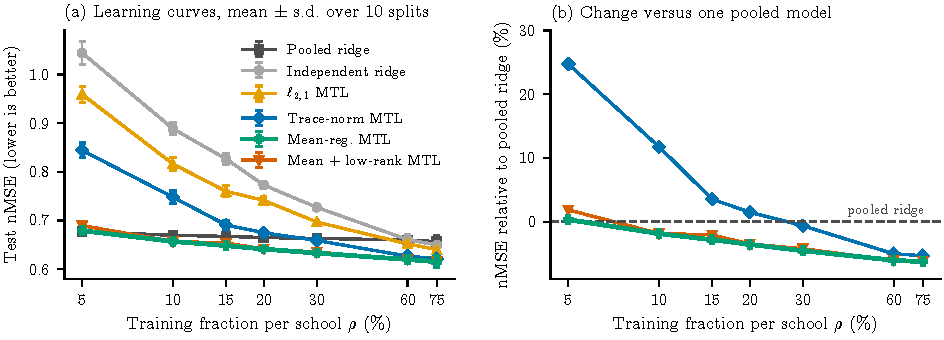
\includegraphics[width=\textwidth]{fig2_learning_curves.pdf}
\caption{Test nMSE as a function of the training fraction per school (log scale). (a) Absolute error; error bars are one standard deviation over 10 splits. (b) Error relative to pooled ridge for the three strongest multi-task methods; negative values beat the pooled model. Trace-norm MTL overtakes pooled ridge only between 20\% and 30\%, whereas mean-regularized MTL (thick green) is at or below the pooled model at every training fraction.}
\label{fig:curves}
\end{figure}

\begin{table}[t]
\centering
\caption{Test nMSE (MSE divided by the variance of test scores; lower is better) as a function of the training fraction per school $\rho$. Mean $\pm$ s.d.\ over 10 random splits; best in bold, second best underlined.}
\label{tab:main}
\small
\setlength{\tabcolsep}{3.6pt}
\begin{tabular}{@{}lccccccc@{}}
\toprule
& \multicolumn{7}{c}{Training fraction per school $\rho$} \\
\cmidrule(l){2-8}
Method & 5\% & 10\% & 15\% & 20\% & 30\% & 60\% & 75\% \\
\midrule
Pooled ridge & \textbf{.677}\,{\scriptsize$\pm$.004} & .669\,{\scriptsize$\pm$.003} & .667\,{\scriptsize$\pm$.001} & .665\,{\scriptsize$\pm$.002} & .663\,{\scriptsize$\pm$.004} & .660\,{\scriptsize$\pm$.008} & .656\,{\scriptsize$\pm$.013} \\
Independent ridge & 1.045\,{\scriptsize$\pm$.023} & .889\,{\scriptsize$\pm$.012} & .826\,{\scriptsize$\pm$.012} & .773\,{\scriptsize$\pm$.006} & .727\,{\scriptsize$\pm$.004} & .660\,{\scriptsize$\pm$.009} & .649\,{\scriptsize$\pm$.012} \\
\midrule
$\ell_{2,1}$ MTL & .959\,{\scriptsize$\pm$.016} & .816\,{\scriptsize$\pm$.014} & .760\,{\scriptsize$\pm$.011} & .741\,{\scriptsize$\pm$.007} & .697\,{\scriptsize$\pm$.004} & .652\,{\scriptsize$\pm$.006} & .640\,{\scriptsize$\pm$.012} \\
Trace-norm MTL & .844\,{\scriptsize$\pm$.015} & .748\,{\scriptsize$\pm$.013} & .691\,{\scriptsize$\pm$.010} & .675\,{\scriptsize$\pm$.004} & .659\,{\scriptsize$\pm$.003} & .626\,{\scriptsize$\pm$.007} & .621\,{\scriptsize$\pm$.012} \\
\midrule
Mean-reg.\ MTL & \underline{.679}\,{\scriptsize$\pm$.008} & \textbf{.657}\,{\scriptsize$\pm$.004} & \textbf{.648}\,{\scriptsize$\pm$.002} & \textbf{.641}\,{\scriptsize$\pm$.003} & \textbf{.633}\,{\scriptsize$\pm$.004} & \underline{.620}\,{\scriptsize$\pm$.008} & \textbf{.615}\,{\scriptsize$\pm$.012} \\
Mean + low-rank MTL & .689\,{\scriptsize$\pm$.007} & \underline{.657}\,{\scriptsize$\pm$.003} & \underline{.653}\,{\scriptsize$\pm$.003} & \underline{.641}\,{\scriptsize$\pm$.002} & \underline{.635}\,{\scriptsize$\pm$.004} & \textbf{.619}\,{\scriptsize$\pm$.008} & \underline{.616}\,{\scriptsize$\pm$.013} \\
\bottomrule
\end{tabular}
\end{table}

\begin{table}[t]
\centering
\caption{Paired comparisons on the same splits. Each cell gives the relative nMSE change of the first method against the second (\%, negative means the first method is better) and, in parentheses, the number of the 10 splits on which the first method wins. $^{\dagger}$: two-sided $p < 0.05$ under the corrected resampled $t$-test of \citet{nadeau2003inference}, which is conservative when the test set is much larger than the training set (small $\rho$). Indep.: independent ridge; Pooled: pooled ridge; Trace: trace-norm MTL; MR: mean-regularized MTL; MLR: mean + low-rank MTL.}
\label{tab:paired}
\footnotesize
\setlength{\tabcolsep}{4.2pt}
\begin{tabular}{@{}lccccccc@{}}
\toprule
& \multicolumn{7}{c}{Training fraction per school $\rho$} \\
\cmidrule(l){2-8}
Comparison & 5\% & 10\% & 15\% & 20\% & 30\% & 60\% & 75\% \\
\midrule
Trace vs.\ Indep. & $-19.2$\,{\scriptsize(10)} & $-15.9$$^{\dagger}$\,{\scriptsize(10)} & $-16.4$$^{\dagger}$\,{\scriptsize(10)} & $-12.7$$^{\dagger}$\,{\scriptsize(10)} & $-9.4$$^{\dagger}$\,{\scriptsize(10)} & $-5.2$$^{\dagger}$\,{\scriptsize(10)} & $-4.4$$^{\dagger}$\,{\scriptsize(10)} \\
Trace vs.\ Pooled & $+24.7$$^{\dagger}$\,{\scriptsize(0)} & $+11.7$\,{\scriptsize(0)} & $+3.5$\,{\scriptsize(0)} & $+1.5$\,{\scriptsize(0)} & $-0.7$\,{\scriptsize(8)} & $-5.0$$^{\dagger}$\,{\scriptsize(10)} & $-5.3$$^{\dagger}$\,{\scriptsize(10)} \\
MR vs.\ Pooled & $+0.3$\,{\scriptsize(4)} & $-1.9$\,{\scriptsize(10)} & $-2.8$$^{\dagger}$\,{\scriptsize(10)} & $-3.6$$^{\dagger}$\,{\scriptsize(10)} & $-4.6$$^{\dagger}$\,{\scriptsize(10)} & $-6.1$$^{\dagger}$\,{\scriptsize(10)} & $-6.3$$^{\dagger}$\,{\scriptsize(10)} \\
MR vs.\ Trace & $-19.6$\,{\scriptsize(10)} & $-12.2$\,{\scriptsize(10)} & $-6.1$\,{\scriptsize(10)} & $-5.0$$^{\dagger}$\,{\scriptsize(10)} & $-3.9$$^{\dagger}$\,{\scriptsize(10)} & $-1.1$\,{\scriptsize(9)} & $-1.0$$^{\dagger}$\,{\scriptsize(10)} \\
MLR vs.\ Pooled & $+1.8$\,{\scriptsize(1)} & $-1.9$\,{\scriptsize(10)} & $-2.1$\,{\scriptsize(10)} & $-3.5$$^{\dagger}$\,{\scriptsize(10)} & $-4.3$$^{\dagger}$\,{\scriptsize(10)} & $-6.1$$^{\dagger}$\,{\scriptsize(10)} & $-6.1$$^{\dagger}$\,{\scriptsize(10)} \\
MLR vs.\ Trace & $-18.3$$^{\dagger}$\,{\scriptsize(10)} & $-12.2$$^{\dagger}$\,{\scriptsize(10)} & $-5.4$\,{\scriptsize(10)} & $-4.9$$^{\dagger}$\,{\scriptsize(10)} & $-3.6$$^{\dagger}$\,{\scriptsize(10)} & $-1.1$\,{\scriptsize(10)} & $-0.8$$^{\dagger}$\,{\scriptsize(10)} \\
MLR vs.\ MR & $+1.5$\,{\scriptsize(0)} & $+0.0$\,{\scriptsize(3)} & $+0.8$\,{\scriptsize(1)} & $+0.1$\,{\scriptsize(4)} & $+0.3$\,{\scriptsize(0)} & $-0.0$\,{\scriptsize(4)} & $+0.1$\,{\scriptsize(2)} \\
\bottomrule
\end{tabular}
\end{table}


\Cref{fig:curves} and \cref{tab:main} show how each method behaves as the training fraction grows from 5\% to 75\%. The usual multi-task story holds against independent models: trace-norm MTL beats independent ridge on all 10 splits at every training fraction, by 19.2\% in nMSE at 5\% and 4.4\% at 75\%, and $\ell_{2,1}$ MTL sits between the two (\cref{tab:paired}).

The pooled model tells a different story. Its error barely changes with the amount of data (nMSE 0.677 at 5\% and 0.656 at 75\%), because the part of the scores it cannot explain is school-specific. Yet at small training fractions it beats every per-school method. Trace-norm MTL is worse than pooled ridge on all 10 splits up to 20\% training, by 24.7\% at 5\% and still 1.5\% at 20\%. It overtakes the pooled model between 20\% and 30\% (better on 8 of 10 splits at 30\%) and is clearly better only at 60\% and 75\% (10 of 10 splits, about 5\%). Independent ridge does not beat the pooled model until 75\%.

\subsection{Why the pooled model wins}
\label{sec:res-why}

Two properties combine. The first is in the data. Seven columns, including the bias, are constant within every school (\cref{sec:setup}), so a model fitted to one school can only estimate their combined effect as an intercept, and the separate effects of school-level attributes are identifiable only across schools. The pooled model estimates these shared effects with all 15,362 students, while each school-specific model must estimate its own intercept from as few as one training student at $\rho = 5\%$.

The second is in the regularizers. Multi-task penalties do share information, but their shrinkage target is zero (\cref{prop:limits}), so when data are scarce and cross-validation selects strong regularization, the part all schools have in common is shrunk along with the rest. We can measure this directly. At $\rho = 5\%$ the average school model under trace-norm MTL has $57 \pm 4\%$ of the Euclidean norm of the pooled model, rising to $69\%$ at 20\% and $74\%$ at 75\%. Under mean-regularized MTL the same ratio is $134 \pm 25\%$ at 5\% and $95 \pm 4\%$ at 75\%: the shared model is not shrunk. \Cref{fig:overview} shows the learned matrices: trace-norm MTL keeps the pooled model's pattern of weights but pales it, while the mean + low-rank model reproduces the pooled weights and adds small school-specific deviations.

\subsection{Partial pooling}
\label{sec:res-partial}

Mean-regularized MTL resolves the trade-off (\cref{tab:main,tab:paired}). At 5\% training it is statistically indistinguishable from pooled ridge (0.3\% worse on average, winning 4 of 10 splits). From 10\% onwards it beats pooled ridge on all 10 splits at every training fraction, by 1.9\% at 10\% rising to 6.3\% at 75\%, significant under the corrected test from 15\% onwards. It also has lower error than trace-norm MTL at every training fraction, by 19.6\% at 5\%, 5.0\% at 20\% and 1.0\% at 75\%, winning on at least 9 of 10 splits each time. It is the best method at every training fraction except 5\%, where pooled ridge is marginally ahead, and 60\%, where the mean + low-rank model is ahead by 0.04\%.

Restricting the deviations to be low rank does not help. From 10\% onwards the two partial-pooling estimators are within 0.8\% of each other. At 5\% the mean + low-rank model is 1.5\% worse than mean-regularized MTL: cross-validation removes its deviations entirely on 7 of the 10 splits, reducing it to the school-weighted pooled model of \cref{prop:limits}, and overall it is 1.8\% worse than the student-weighted pooled ridge. With one or two training students in many schools, giving every school equal weight in \eqref{eq:loss} discards information that pooled ridge keeps.

\subsection{Who benefits}
\label{sec:res-who}

\begin{figure}[t]
\centering
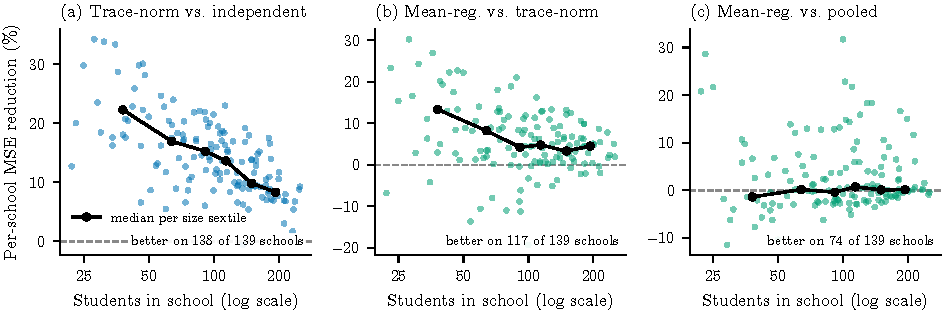
\includegraphics[width=\textwidth]{fig3_per_school.pdf}
\caption{Per-school change in test MSE at $\rho = 20\%$, averaged over 10 splits; positive values mean the first-named method is better. Each dot is one school, plotted against its size; the black line joins the median within six size groups. Sharing helps small schools most (a, b), while the gain of partial pooling over the pooled model is concentrated in a minority of schools of all sizes (c).}
\label{fig:per-school}
\end{figure}

\Cref{fig:per-school} breaks the gains down by school at $\rho = 20\%$. Trace-norm MTL improves on independent ridge for 138 of the 139 schools, and the improvement shrinks with school size (Spearman correlation $-0.63$): the median reduction in MSE is 17.6\% for schools below the median size and 10.4\% above it. Mean-regularized MTL improves on trace-norm MTL for 117 schools, again more for small schools (median 8.3\% against 4.5\%, Spearman $-0.27$, $p = 0.001$). Its 3.6\% advantage over the pooled model is distributed differently: it is better for only 74 of the 139 schools, with no relation to size (Spearman $0.10$, $p = 0.26$). The aggregate gain comes from a minority of schools that the pooled model fits poorly, several of which see reductions of 10 to 30\%.

\subsection{What structure is learned}
\label{sec:res-structure}

\begin{figure}[t]
\centering
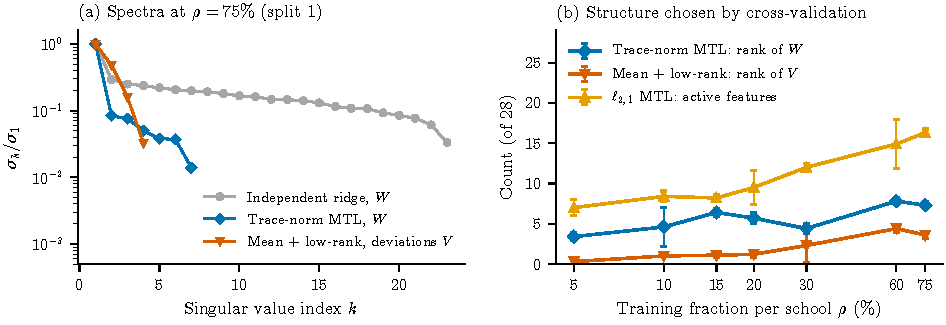
\includegraphics[width=\textwidth]{fig4_structure.pdf}
\caption{(a) Normalized singular values of the learned models at $\rho = 75\%$ (first split): the independent models, the trace-norm model and the deviations of the mean + low-rank model. (b) Structure selected by cross-validation as the training fraction grows: rank of the trace-norm model, rank of the mean + low-rank deviations and number of features kept by $\ell_{2,1}$ MTL (mean $\pm$ s.d.\ over 10 splits).}
\label{fig:structure}
\end{figure}

\Cref{fig:structure}a shows that the independent models do not share a low-dimensional subspace on their own: their singular values decay slowly ($\sigma_2/\sigma_1 = 0.29$) over a rank of 23. The trace-norm model concentrates almost all of its energy in one direction ($\sigma_2/\sigma_1 = 0.08$, rank 7), consistent with a dominant shared component. Once that component is modeled explicitly as a mean, the deviations need only a few directions (rank 4 in this split). \Cref{fig:structure}b shows that the selected structure grows with the data: $\ell_{2,1}$ MTL keeps 7 of 28 features at 5\% and 16 at 75\%, and the rank of the mean + low-rank deviations rises from below 1 on average at 5\% to about 4 at 60\% and 75\%. The rank of the trace-norm model changes less regularly, between 3 and 8, because the same directions must carry both the shared and the school-specific parts.

\subsection{Optimization: a fixed budget fails silently on unscaled features}
\label{sec:res-optim}

\begin{figure}[t]
\centering
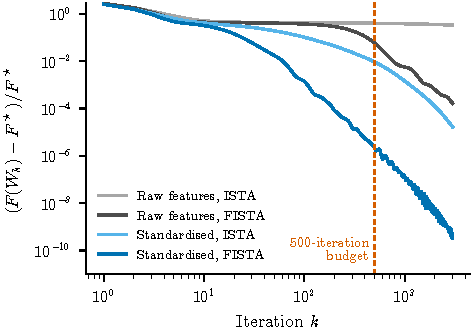
\includegraphics[width=0.56\textwidth]{fig5_optimisation.pdf}
\caption{Relative suboptimality of trace-norm MTL ($\lambda = 3$, $\rho = 75\%$, first split) for proximal gradient without (ISTA) and with (FISTA) momentum, on raw and standardized features. The dashed line marks the 500-iteration budget.}
\label{fig:optim}
\end{figure}

On raw features the two numeric columns take values up to 91 and 43, and the Lipschitz constant of the loss gradient is $L = 8{,}296$. Since the step size is $1/L$, progress per iteration is tiny: after 500 iterations FISTA is still 5.9\% above the optimal objective and ISTA 41\% above (\cref{fig:optim}). Standardizing the two columns lowers $L$ to 24.5, and FISTA then reaches a relative gap of $2.2 \times 10^{-6}$ within the same budget. Nothing in the output signals the difference, so fixed-budget solvers on unscaled data can produce unconverged models whose errors are then attributed to the method. All results in this paper use standardized features, and acceleration matters as well: on standardized features ISTA is still $9.4 \times 10^{-3}$ above the optimum after 500 iterations.

\subsection{Metric definitions change reported numbers}
\label{sec:res-metrics}

Explained variance on School is reported with two normalizations: by the variance of all test scores, or by the average variance within schools as in \eqref{eq:ev}. For identical predictions the two differ by 11.1 to 13.0 points (\cref{tab:metrics}): trace-norm MTL scores 26.5\% under the within-school definition and 37.9\% under the pooled one. The pooled definition credits a model for explaining differences between schools, which make up 11.5\% of the variance. Rankings are unchanged, but absolute values are not comparable across papers that normalize differently, and published numbers should be compared only after the definition is confirmed.

\section{Discussion}
\label{sec:discussion}

\paragraph{Shrink towards a common model, not towards zero.}
The $\ell_{2,1}$ and trace-norm penalties share information between tasks, but their shrinkage target is the zero matrix (\cref{prop:limits}). When data are scarce, cross-validation chooses strong regularization, and the estimate of the part all schools have in common is shrunk along with everything else. Pooled ridge makes the opposite error: it estimates the common part with all the data and ignores school-specific effects. Partial pooling estimates the common part almost without penalty and spends the regularization budget only on deviations from it. On School this is enough to match the pooled model when schools have a handful of students and to beat every alternative once they have more. A trace-norm model can represent a shared mean as one of its directions, so the difference is not one of expressiveness but of where the penalty is applied. The behaviour of the partial-pooling estimators, close to pooling with little data and ahead of it with more, is what the adaptivity results of \citet{duan2023adaptive} predict for estimators that shrink towards a learned center.

\paragraph{Relation to earlier School results.}
At $\rho = 75\%$ our results agree with \citet{argyriou2008convex}: the pooled model explains 22.0\% of within-school variance against their 22.7\%, clearly below trace-norm MTL. They disagree with \citet{evgeniou2005kernel}, who found a single model for all schools best under the same protocol. Their models were support vector regressions rather than ridge regressions, and we did not reproduce their setup, so we cannot say which difference explains the disagreement. Neither study examined small training fractions, which is where, in our experiments, the pooled model is strongest and the choice between shrinking towards zero and shrinking towards a common model matters most.

\paragraph{Structure in the deviations.}
Constraining the deviations to be low rank does not help on School: from 10\% training onwards the two partial-pooling estimators are within 0.8\% of each other, and at 5\% the low-rank variant is worse (\cref{tab:main}). The rank that cross-validation selects for the deviations grows with the data (\cref{fig:structure}b), which suggests that schools differ along a few directions beyond their intercept, but these differences carry little predictive weight relative to the shared model and the noise. We expect structured deviations to matter more where task differences are larger than the 11.5\% between-school share of variance seen here.

\paragraph{Recommendations for evaluating multi-task models.}
Three practices would have changed the conclusions drawn from School. First, report a pooled model and a partial-pooling model alongside independent models; both are cheap, and the pooled model is the natural null hypothesis when tasks share features. Second, report results over a range of training fractions, since the ranking of methods reverses between 20\% and 30\% (\cref{fig:curves}). Third, state the metric exactly, including how variance is normalized, and check optimizer convergence rather than relying on an iteration budget.

\paragraph{Limitations.}
We study a single benchmark with linear models and squared loss, so we make no claim about other datasets, nonlinear models or classification. Our splits are random per-school splits that follow the published protocols but are not the published splits, which may explain small differences in \cref{tab:repro}. We did not re-implement learned task-relationship methods such as MTRL \citep{zhang2010convex} or GO-MTL \citep{kumar2012learning}; their published numbers suggest gains beyond trace-norm MTL, and combining them with a shared mean is a natural next step. Our hyperparameters are chosen by cross-validation inside each training set, whereas some published results use a separate validation set. Finally, the corrected resampled $t$-test is conservative at small training fractions, so some differences that win on all 10 splits are not marked significant.


\section{Conclusion}
\label{sec:conclusion}
On the School benchmark, the advantage of regularized multi-task learning depends on which baseline it is compared with. Against independent per-school models, trace-norm and $\ell_{2,1}$ MTL win at every data size. Against a single pooled model, they lose whenever schools have little data, because their penalties shrink every school towards zero instead of towards what the schools have in common. Partial pooling, which learns a shared mean and regularizes only the deviations from it, removes this weakness: mean-regularized MTL matches the pooled model at the smallest data size and is the best or tied-best of the methods we tested from 10\% training onwards. Earlier work on School already found pooling hard to beat at one data size \citep{evgeniou2005kernel}; across data sizes, we suggest that pooled and partial-pooling baselines become standard when linear multi-task methods are compared.

\section*{Reproducibility Statement}
The code repository \texttt{shrink-towards-the-mean}, linked from the archived record of this report, contains everything needed to reproduce it: the proximal-gradient implementation, the benchmark harness, the partial-pooling estimators, the optimization experiment, the analysis, and the scripts that generate every figure and table. They use only NumPy, SciPy and Matplotlib, read the School data as distributed with MALSAR \citep{zhou2011malsar}, fix all random seeds, and reproduce every table and figure with one command (\texttt{python run\_all.py}) in about 25 minutes on two CPU cores. A verification script checks a fresh run against the stored results; on our machine the rerun matched them exactly. Every number in the tables is generated by script from the stored results.

\section*{Acknowledgements}
The author thanks the MALSAR authors for distributing the School data in a convenient form.

\bibliographystyle{plainnat}
\bibliography{references}

\clearpage
\appendix
\section{Additional Results}
\label{app:extra}

\begin{table}[h]
\centering
\caption{The same predictions ($\rho = 75\%$) scored under two definitions of explained variance and under nMSE. Pooled EV uses the variance of all test scores; within-school EV uses the average within-school variance, as in \citet{argyriou2008convex}.}
\label{tab:metrics}
\small
\begin{tabular}{@{}lccc@{}}
\toprule
Method & EV within schools (\%) & EV pooled (\%) & nMSE \\
\midrule
Pooled ridge & $22.0 \pm 1.6$ & $34.4 \pm 1.3$ & $0.6562 \pm 0.0130$ \\
Independent ridge & $22.1 \pm 1.8$ & $35.1 \pm 1.2$ & $0.6494 \pm 0.0116$ \\
$\ell_{2,1}$ MTL & $23.6 \pm 1.8$ & $36.0 \pm 1.2$ & $0.6398 \pm 0.0121$ \\
Trace-norm MTL & $26.5 \pm 1.5$ & $37.9 \pm 1.2$ & $0.6211 \pm 0.0122$ \\
Mean-reg.\ MTL & $27.3 \pm 1.5$ & $38.5 \pm 1.2$ & $0.6150 \pm 0.0123$ \\
Mean + low-rank MTL & $27.3 \pm 1.5$ & $38.4 \pm 1.3$ & $0.6159 \pm 0.0126$ \\
\bottomrule
\end{tabular}
\end{table}

\begin{table}[h]
\centering
\caption{Hyperparameter grids (log-spaced; number of values in parentheses) and the median value selected by 5-fold cross-validation at each training fraction. Across all 420 selections, 0 fell on the boundary of a grid.}
\label{tab:hyper}
\footnotesize
\setlength{\tabcolsep}{3.2pt}
\begin{tabular}{@{}llccccccc@{}}
\toprule
Method & Grid (values) & 5\% & 10\% & 15\% & 20\% & 30\% & 60\% & 75\% \\
\midrule
Pooled ridge & $\mu$: $10^{-6}$ to $10^{2}$ (17) & 0.01 & 0.01 & $3.2\cdot 10^{-3}$ & $3.2\cdot 10^{-3}$ & $3.2\cdot 10^{-3}$ & $6.6\cdot 10^{-4}$ & $3.2\cdot 10^{-5}$ \\
Independent ridge & $\mu$: $10^{-6}$ to $10^{2}$ (17) & 0.32 & 0.32 & 0.32 & 0.1 & 0.1 & 0.032 & 0.032 \\
$\ell_{2,1}$ MTL & $\lambda$: $10^{-1.5}$ to $10^{2.5}$ (12) & 26 & 11 & 11 & 11 & 4.8 & 2.1 & 2.1 \\
Trace-norm MTL & $\lambda$: $10^{-1.5}$ to $10^{2.5}$ (12) & 26 & 18 & 11 & 11 & 11 & 4.8 & 4.8 \\
Mean-reg.\ MTL & $\lambda$: $10^{-4}$ to $10^{3}$ (15) & 32 & 10 & 10 & 3.2 & 3.2 & 1 & 1 \\
Mean + low-rank MTL & $\lambda$: $10^{-2.5}$ to $10^{3.5}$ (15) & 164 & 61 & 61 & 23 & 23 & 8.5 & 8.5 \\
\bottomrule
\end{tabular}
\end{table}


\paragraph{Per-school analysis.}
\Cref{fig:per-school} uses the 20\% training fraction. For every school we average its test MSE over the 10 splits under each method and report the relative reduction against a baseline. The black line connects the median reduction within six groups of schools of increasing size.

\paragraph{Optimization experiment.}
\Cref{fig:optim} uses the first split of the 75\% protocol and $\lambda = 3$. The reference value $F^\star$ for each feature scaling is the best objective found in 100,000 FISTA iterations.
\end{document}
